\documentclass[preprint,12pt,aps,pra,showkeys,amsmath,amssymb,superscriptaddress,floatfix]{revtex4-2}
\usepackage[T1]{fontenc}
\usepackage[utf8]{inputenc}
\usepackage{amsmath,amssymb,amsthm,mathtools,mathrsfs}
\usepackage{microtype,booktabs,enumitem}
\usepackage{xcolor,tikz,etoolbox}
\usepackage[skins,breakable]{tcolorbox}
\usepackage{needspace}
% Keep diagram geometry independent of REVTeX preprint body spacing.
\AtBeginEnvironment{tikzpicture}{\linespread{1}\selectfont}
\usetikzlibrary{arrows.meta,positioning,calc,fit,decorations.pathreplacing}
\usepackage{graphicx}
\usepackage{hyperref}

\definecolor{MMBlue}{RGB}{0,82,155}
\definecolor{MMOrange}{RGB}{200,80,0}
\tikzset{
 mmnode/.style={draw=MMBlue,rounded corners=2pt,fill=MMBlue!4,align=left,execute at begin node={\raggedright},text width=5cm,font=\fontsize{10}{12}\selectfont,inner sep=6pt},
 mmimport/.style={mmnode,draw=black!65,fill=black!4},
 mmcandidate/.style={mmnode,draw=MMOrange,dashed,fill=MMOrange!5},
 mmrejected/.style={mmnode,draw=black,densely dotted,fill=black!8},
 mmproof/.style={->,thick,MMBlue},
 mmflow/.style={->,semithick,black!70},
 mmrepair/.style={->,dashed,thick,MMOrange},
 mmcandidatearrow/.style={->,dashed,semithick,MMOrange},
 mmnote/.style={font=\scriptsize,fill=white,inner sep=2pt,align=center}}

\usepackage[section]{placeins}
\setlength{\emergencystretch}{3em}
\setlist{itemsep=3pt,topsep=4pt}
\newtheorem{theorem}{Theorem}[section]
\newtheorem{proposition}[theorem]{Proposition}
\newtheorem{lemma}[theorem]{Lemma}
\newtheorem{corollary}[theorem]{Corollary}
\theoremstyle{definition}
\newtheorem{definition}[theorem]{Definition}
\newtheorem{example}[theorem]{Example}
\theoremstyle{remark}
\newtheorem{remark}[theorem]{Remark}
% Avoid isolated statement headings and single-line paragraph fragments.
\BeforeBeginEnvironment{theorem}{\Needspace{6\baselineskip}}
\BeforeBeginEnvironment{definition}{\Needspace{5\baselineskip}}
\BeforeBeginEnvironment{proposition}{\Needspace{5\baselineskip}}
\BeforeBeginEnvironment{lemma}{\Needspace{5\baselineskip}}
\BeforeBeginEnvironment{corollary}{\Needspace{5\baselineskip}}
\clubpenalty=5000
\widowpenalty=5000
\newcommand{\R}{\mathbb R}\newcommand{\Z}{\mathbb Z}\newcommand{\N}{\mathbb N}
\newcommand{\Pa}{\operatorname{Pa}}\newcommand{\Desc}{\operatorname{Desc}}
\newcommand{\cl}{\operatorname{cl}}\newcommand{\cost}{\operatorname{cost}}
\newcommand{\status}{\operatorname{status}}
% Faculty cards: a visual rail groups the five faculties within one agent.
% The rail has no arrowhead and does not represent a proof dependency.
\newcommand{\mmfacultybadge}[1]{%
 \node[circle,draw=MMBlue,line width=1pt,fill=white,
 minimum size=7mm,inner sep=0pt,font=\sffamily\small\bfseries,text=MMBlue]
 at ([xshift=15pt,yshift=-15pt]frame.north west) {#1};}
\newcommand{\mmfacultyrail}{%
 \draw[MMBlue!80,line width=1pt]
 ([xshift=15pt,yshift=2pt]frame.north west)--
 ([xshift=15pt,yshift=-2pt]frame.south west);}
\newtcolorbox{mmfacultybox}[2]{enhanced,breakable,
 colback=MMBlue!4,colframe=MMBlue!4,boxrule=0pt,arc=3pt,
 left=39pt,right=9pt,top=4pt,bottom=4pt,
 before skip=2pt,after skip=2pt,
 fontupper=\small\linespread{1.1}\selectfont,
 overlay unbroken={\mmfacultyrail\mmfacultybadge{#1}},
 overlay first={\mmfacultyrail\mmfacultybadge{#1}},
 overlay middle={\mmfacultyrail},overlay last={\mmfacultyrail}}
\newcommand{\mmfaculty}[3]{%
 \begin{mmfacultybox}{#1}{#2}
 {\sffamily\bfseries\color{MMBlue}#2}\par\smallskip #3
 \end{mmfacultybox}}
\newcommand{\agent}[9]{%
 \Needspace{8\baselineskip}
 \subsubsection{#1}
 \noindent\textbf{Object.} #2\par
 \noindent\textbf{Role.} #3\par\smallskip
 \mmfaculty{E}{Ego}{#4}
 \mmfaculty{M}{Memory}{#5}
 \mmfaculty{I}{Intellect}{#6}
 \mmfaculty{S}{Sense}{#7}
 \mmfaculty{A}{Action}{#8}
 \smallskip\noindent #9\par}

\usepackage{longtable,array,calc}
\providecommand{\tightlist}{\setlength{\itemsep}{2pt}\setlength{\parskip}{0pt}}
\makeatletter
\def\frontmatter@abstract@produce{\par\addvspace{\frontmatter@preabstractspace}%
\begingroup\prep@absbox\unvbox\absbox\post@absbox\endgroup
\addvspace{\frontmatter@postabstractspace}}
\makeatother
\newcommand{\field}[2]{\par\smallskip\noindent\textbf{#1.} #2\par}
\setlength{\emergencystretch}{5em}
\AtBeginEnvironment{verbatim}{\small\linespread{1.0}\selectfont}


\hypersetup{colorlinks=true,linkcolor=MMBlue,urlcolor=MMBlue,pdfauthor={Dibakar Sigdel}}

\begin{document}

\title{Weak Nullstellensatz\\[4pt]\large An End-to-End Meta-Math Walkthrough}

\author{Dibakar Sigdel}

\affiliation{Mindverse Computing LLC, Lynnwood, WA 98087, USA}

\date{October 2026}

\begin{abstract}

A field that is finitely generated as a \(k\)-algebra cannot contain a
transcendental generator: integrality would force a polynomial ring with
only one denominator inverted to be a field. The report presents the
target theorem, declared imports, a dependency graph, five-faculty node
contracts, a continuous proof, a worked example, and a hypothesis-repair
audit. It is an authored mathematical exposition, not a deployed-agent
transcript or a formal proof-assistant certificate.

\end{abstract}\maketitle\linespread{1.12}\selectfont

\noindent\textbf{AG-02 / Algebraic Geometry / Report v1}

\section{Target and import contract}

\begin{theorem}

Let \(k\) be algebraically closed and \(A=k[x_1,\ldots,x_n]\), with
finite \(n\ge0\). Every maximal ideal is \((x_1-a_1,\ldots,x_n-a_n)\)
for a unique point \(a\in k^n\). Consequently every proper ideal of
\(A\) has a common zero in \(k^n\).

\end{theorem}

\subsection{Foundations and permitted imports}

Use existence of maximal ideals containing proper ideals (Zorn's lemma),
finite transcendence bases chosen from a finite generating set, and
elementary field algebra. Import the integrality facts: finitely many
integral elements generate a finite module; every element of a
finite-module algebra is integral, by the determinant trick. An element
is integral over a ring if it satisfies a monic polynomial with
coefficients in that ring. The finite-generation field lemma needed
below is proved here, not imported as the target.

\clearpage\section{Node interaction workflow}

\begin{center}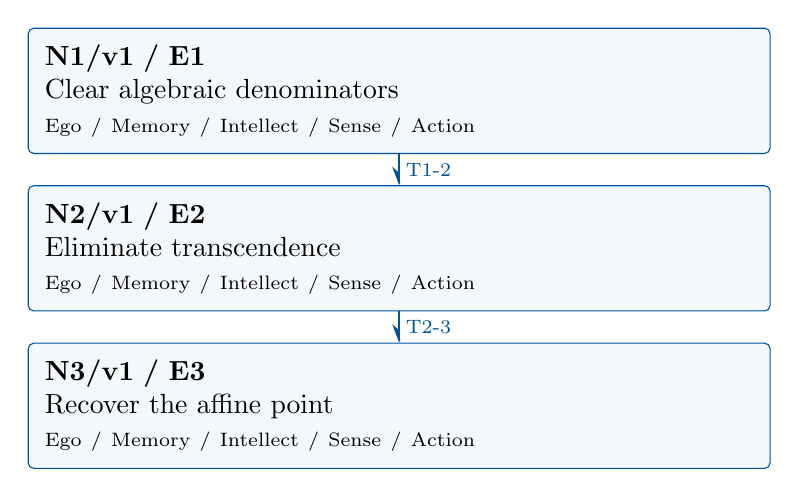
\begin{tikzpicture}[>=Stealth,x=1cm,y=1cm]

\node[mmnode,text width=9cm,minimum height=1.25cm] (N1) at (0,0.0) {\textbf{N1/v1 / E1}\\Clear algebraic denominators\\{\scriptsize Ego / Memory / Intellect / Sense / Action}};

\node[mmnode,text width=9cm,minimum height=1.25cm] (N2) at (0,-2.0) {\textbf{N2/v1 / E2}\\Eliminate transcendence\\{\scriptsize Ego / Memory / Intellect / Sense / Action}};

\node[mmnode,text width=9cm,minimum height=1.25cm] (N3) at (0,-4.0) {\textbf{N3/v1 / E3}\\Recover the affine point\\{\scriptsize Ego / Memory / Intellect / Sense / Action}};

\draw[mmproof] (N1.south) -- node[mmnote,right] {T1-2} (N2.north);

\draw[mmproof] (N2.south) -- node[mmnote,right] {T2-3} (N3.north);

\end{tikzpicture}\end{center}

Each box is one mathematical agent containing all five faculties. Blue
arrows carry the versioned exports listed below. The layout gives a
reading order; only drawn arrows assert dependencies. Diagnostic repair
is separate from the proof DAG.

\subsection{Versioned evidence-transfer ledger}

\begingroup\small\linespread{1.05}\selectfont

\Needspace{5\baselineskip}\field{T1-2: N1/E1/v1 to N2}{For algebraically independent \(t_1,\ldots,t_r\), there is nonzero
\(d\in k[t_1,\ldots,t_r]\) such that \(K\) is integral over
\(B=k[t_1,\ldots,t_r,1/d]\).}

\field{Receiving activity}{N2.1}

\field{Compatibility}{E1/v1, with \(K\) a field integral over the domain \(B\). Check: The
field \(k\) is infinite; choose \(c\) so that \(t_1-c\) does not divide
\(d\).}

\Needspace{5\baselineskip}\field{T2-3: N2/E2/v1 to N3}{\(r=0\), and hence \(K=k\) for every finitely generated \(k\)-algebra
that is a field.}

\field{Receiving activity}{N3.1}

\field{Compatibility}{A maximal ideal \(\mathfrak m\subset A\) and E2/v1 applied to
\(K=A/\mathfrak m\). Check: The quotient is a field because the ideal is
maximal; the scalar identification must respect the given embedding of
\(k\).}

\endgroup

\clearpage\section{Agent roles and five-faculty activities}\begingroup\small\linespread{1.05}\selectfont\setlist{itemsep=1pt,topsep=2pt}

\begingroup\footnotesize\linespread{1.05}\selectfont\let\small\footnotesize

\subsection{N1/v1: Clear algebraic denominators}

\field{Object and role}{Separate a maximal algebraically independent subset and make the
remaining generators integral after one localization. \textbf{Local
obligation:} For algebraically independent \(t_1,\ldots,t_r\), there is
nonzero \(d\in k[t_1,\ldots,t_r]\) such that \(K\) is integral over
\(B=k[t_1,\ldots,t_r,1/d]\).}

\field{Inputs}{A field \(K=k[b_1,\ldots,b_m]\) over the algebraically closed field
\(k\).}

\mmfaculty{E}{Ego}{Publish E1/v1 only after establishing this obligation: For algebraically
independent \(t_1,\ldots,t_r\), there is nonzero
\(d\in k[t_1,\ldots,t_r]\) such that \(K\) is integral over
\(B=k[t_1,\ldots,t_r,1/d]\).}

\mmfaculty{M}{Memory}{A field \(K=k[b_1,\ldots,b_m]\) over the algebraically closed field
\(k\). Retain the stated assumptions and import versions.}

\mmfaculty{I}{Intellect}{Separate a maximal algebraically independent subset and make the
remaining generators integral after one localization.}

\mmfaculty{S}{Sense}{Finite generation is as an algebra, not merely as a field; only finitely
many denominators need to be inverted.}

\mmfaculty{A}{Action}{Carry out activities N1.1--N1.2 below, retaining each calculation and
construction as evidence.}

\smallskip\noindent\textbf{Numbered mathematical activities}

\begin{enumerate}[label=N1.\arabic*,leftmargin=3.4em]

\item Choose a maximal algebraically independent subset \(t_1,\ldots,t_r\) of
the generators. Every remaining generator \(u_j\) is algebraic over
\(F=k(t_1,\ldots,t_r)\): otherwise the subset could be enlarged. Each
\(u_j\) satisfies a monic polynomial over \(F\).

\item Let \(d\ne0\) be the product of the finitely many polynomial
denominators in these monic equations (take \(d=1\) if there are none).
The \(u_j\) are integral over \(B=k[t_1,\ldots,t_r,1/d]\). Because \(K\)
is a field, \(1/d\in K\); because \(K=k[t_1,\ldots,t_r,u_1,\ldots,u_s]\)
as an algebra, \(B[u_1,\ldots,u_s]=K\). The stated integrality facts now
show \(K\) is integral over \(B\).

\end{enumerate}

\field{Export E1/v1}{For algebraically independent \(t_1,\ldots,t_r\), there is nonzero
\(d\in k[t_1,\ldots,t_r]\) such that \(K\) is integral over
\(B=k[t_1,\ldots,t_r,1/d]\).}

\field{Acceptance gate}{Finite generation is as an algebra, not merely as a field; only finitely
many denominators need to be inverted.}

\field{Targeted repair}{If arbitrary rational coefficients are treated as polynomial
coefficients, explicitly collect their finitely many denominators into
\(d\). Withhold this export and recheck its descendants after a
versioned correction.}

\endgroup

\clearpage

\subsection{N2/v1: Eliminate transcendence}

\field{Object and role}{First force \(B\) to be a field, then find a polynomial that cannot
become a unit in that localization. \textbf{Local obligation:} \(r=0\),
and hence \(K=k\) for every finitely generated \(k\)-algebra that is a
field.}

\field{Inputs}{E1/v1, with \(K\) a field integral over the domain \(B\). Incoming proof
exports: E1/v1 at N2.1.}

\mmfaculty{E}{Ego}{Publish E2/v1 only after establishing this obligation: \(r=0\), and
hence \(K=k\) for every finitely generated \(k\)-algebra that is a
field.}

\mmfaculty{M}{Memory}{E1/v1, with \(K\) a field integral over the domain \(B\). Incoming proof
exports: E1/v1 at N2.1. Retain the stated assumptions and import
versions.}

\mmfaculty{I}{Intellect}{First force \(B\) to be a field, then find a polynomial that cannot
become a unit in that localization.}

\mmfaculty{S}{Sense}{The field \(k\) is infinite; choose \(c\) so that \(t_1-c\) does not
divide \(d\).}

\mmfaculty{A}{Action}{Carry out activities N2.1--N2.3 below, retaining each calculation and
construction as evidence.}

\smallskip\noindent\textbf{Numbered mathematical activities}

\begin{enumerate}[label=N2.\arabic*,leftmargin=3.4em]

\item For \(0\ne b\in B\), the element \(b^{-1}\in K\) is integral:
\((b^{-1})^q+c_{q-1}(b^{-1})^{q-1}+\cdots+c_0=0\). Multiplying by
\(b^{q-1}\) expresses \(b^{-1}\) as an element of \(B\). Thus \(B\) is a
field.

\item If \(r\ge1\), choose \(c\in k\) with \(t_1-c\nmid d\). Such a \(c\)
exists because a nonzero polynomial has only finitely many distinct
factors \(t_1-c\), whereas an algebraically closed field is infinite. If
\(t_1-c\) were invertible in \(B\), then \((t_1-c)q=d^s\) for some
polynomial \(q\) and integer \(s\ge0\). Substituting \(t_1=c\) gives a
contradiction since \(d(c,t_2,\ldots,t_r)\ne0\). Thus \(B\) would not be
a field. Therefore \(r=0\).

\item All generators are now algebraic over \(k\), and finitely many algebraic
generators give a finite algebraic extension. Algebraic closedness
implies that extension is \(k\) itself. This proves the required
finite-generation field lemma for this base field.

\end{enumerate}

\field{Export E2/v1}{\(r=0\), and hence \(K=k\) for every finitely generated \(k\)-algebra
that is a field.}

\field{Acceptance gate}{The field \(k\) is infinite; choose \(c\) so that \(t_1-c\) does not
divide \(d\).}

\field{Targeted repair}{If the localization is declared a field without proof, derive inverses
from monic equations; if transcendence is ignored, use the nonunit
\(t_1-c\) witness. Withhold this export and recheck its descendants
after a versioned correction.}

\clearpage

\subsection{N3/v1: Recover the affine point}

\field{Object and role}{Identify each coordinate residue with a scalar and identify the kernel
of evaluation. \textbf{Local obligation:} Maximal ideals are exactly
point ideals, and every proper ideal has a common zero.}

\field{Inputs}{A maximal ideal \(\mathfrak m\subset A\) and E2/v1 applied to
\(K=A/\mathfrak m\). Incoming proof exports: E2/v1 at N3.1.}

\mmfaculty{E}{Ego}{Publish E3/v1 only after establishing this obligation: Maximal ideals
are exactly point ideals, and every proper ideal has a common zero.}

\mmfaculty{M}{Memory}{A maximal ideal \(\mathfrak m\subset A\) and E2/v1 applied to
\(K=A/\mathfrak m\). Incoming proof exports: E2/v1 at N3.1. Retain the
stated assumptions and import versions.}

\mmfaculty{I}{Intellect}{Identify each coordinate residue with a scalar and identify the kernel
of evaluation.}

\mmfaculty{S}{Sense}{The quotient is a field because the ideal is maximal; the scalar
identification must respect the given embedding of \(k\).}

\mmfaculty{A}{Action}{Carry out activities N3.1--N3.3 below, retaining each calculation and
construction as evidence.}

\smallskip\noindent\textbf{Numbered mathematical activities}

\begin{enumerate}[label=N3.\arabic*,leftmargin=3.4em]

\item The field \(A/\mathfrak m\) is generated as a \(k\)-algebra by the
coordinate residues. E2 identifies it with \(k\) as a \(k\)-algebra.
Write the residue of \(x_i\) as \(a_i\). Then every
\(x_i-a_i\in\mathfrak m\).

\item Evaluation at \(a\) has kernel \((x_1-a_1,\ldots,x_n-a_n)\): repeatedly
replace coordinates by their values, so \(f(x)-f(a)\) is a sum of
multiples of \(x_i-a_i\). That point ideal is maximal, since evaluation
has quotient \(k\), and inclusion forces equality with \(\mathfrak m\).
Uniqueness follows by comparing coordinate values.

\item If \(I\) is proper, place it inside a maximal ideal and use its point
\(a\). Every polynomial in \(I\) vanishes at \(a\). For \(n=0\), the
only proper ideal of \(k\) is zero, and the unique empty coordinate
tuple gives the same statement.

\end{enumerate}

\field{Export E3/v1}{Maximal ideals are exactly point ideals, and every proper ideal has a
common zero.}

\field{Acceptance gate}{The quotient is a field because the ideal is maximal; the scalar
identification must respect the given embedding of \(k\).}

\field{Targeted repair}{If a nonmaximal ideal is treated as having a field quotient, first pass
to a maximal ideal containing it. Withhold this export and recheck its
descendants after a versioned correction.}

\endgroup\clearpage\section{Continuous mathematical proof}\label{sec:proof}

\subsection{N1 --- Clear algebraic
denominators}\label{n1-clear-algebraic-denominators}

\begin{enumerate}
\def\labelenumi{\arabic{enumi}.}
\item
  \textbf{N1.1.} Choose a maximal algebraically independent subset
  \(t_1,\ldots,t_r\) of the generators. Every remaining generator
  \(u_j\) is algebraic over \(F=k(t_1,\ldots,t_r)\): otherwise the
  subset could be enlarged. Each \(u_j\) satisfies a monic polynomial
  over \(F\).
\item
  \textbf{N1.2.} Let \(d\ne0\) be the product of the finitely many
  polynomial denominators in these monic equations (take \(d=1\) if
  there are none). The \(u_j\) are integral over
  \(B=k[t_1,\ldots,t_r,1/d]\). Because \(K\) is a field, \(1/d\in K\);
  because \(K=k[t_1,\ldots,t_r,u_1,\ldots,u_s]\) as an algebra,
  \(B[u_1,\ldots,u_s]=K\). The stated integrality facts now show \(K\)
  is integral over \(B\).
\end{enumerate}

\subsection{N2 --- Eliminate
transcendence}\label{n2-eliminate-transcendence}

\begin{enumerate}
\def\labelenumi{\arabic{enumi}.}
\item
  \textbf{N2.1.} For \(0\ne b\in B\), the element \(b^{-1}\in K\) is
  integral: \((b^{-1})^q+c_{q-1}(b^{-1})^{q-1}+\cdots+c_0=0\).
  Multiplying by \(b^{q-1}\) expresses \(b^{-1}\) as an element of
  \(B\). Thus \(B\) is a field.
\item
  \textbf{N2.2.} If \(r\ge1\), choose \(c\in k\) with \(t_1-c\nmid d\).
  Such a \(c\) exists because a nonzero polynomial has only finitely
  many distinct factors \(t_1-c\), whereas an algebraically closed field
  is infinite. If \(t_1-c\) were invertible in \(B\), then
  \((t_1-c)q=d^s\) for some polynomial \(q\) and integer \(s\ge0\).
  Substituting \(t_1=c\) gives a contradiction since
  \(d(c,t_2,\ldots,t_r)\ne0\). Thus \(B\) would not be a field.
  Therefore \(r=0\).
\item
  \textbf{N2.3.} All generators are now algebraic over \(k\), and
  finitely many algebraic generators give a finite algebraic extension.
  Algebraic closedness implies that extension is \(k\) itself. This
  proves the required finite-generation field lemma for this base field.
\end{enumerate}

\subsection{N3 --- Recover the affine
point}\label{n3-recover-the-affine-point}

\begin{enumerate}
\def\labelenumi{\arabic{enumi}.}
\item
  \textbf{N3.1.} The field \(A/\mathfrak m\) is generated as a
  \(k\)-algebra by the coordinate residues. E2 identifies it with \(k\)
  as a \(k\)-algebra. Write the residue of \(x_i\) as \(a_i\). Then
  every \(x_i-a_i\in\mathfrak m\).
\item
  \textbf{N3.2.} Evaluation at \(a\) has kernel
  \((x_1-a_1,\ldots,x_n-a_n)\): repeatedly replace coordinates by their
  values, so \(f(x)-f(a)\) is a sum of multiples of \(x_i-a_i\). That
  point ideal is maximal, since evaluation has quotient \(k\), and
  inclusion forces equality with \(\mathfrak m\). Uniqueness follows by
  comparing coordinate values.
\item
  \textbf{N3.3.} If \(I\) is proper, place it inside a maximal ideal and
  use its point \(a\). Every polynomial in \(I\) vanishes at \(a\). For
  \(n=0\), the only proper ideal of \(k\) is zero, and the unique empty
  coordinate tuple gives the same statement.
\end{enumerate}

\hfill$\square$

\section{Worked orchestration}

Over \(\mathbb C\), take \(I=(x^2+1,y-x)\). The points \((i,i)\) and
\((-i,-i)\) both annihilate \(I\). A maximal ideal above \(I\) can be
\((x-i,y-i)\); the theorem guarantees a point for each maximal ideal,
not uniqueness of the common zero of an arbitrary proper ideal.

\subsection{Boundary and hypothesis audit}

Over \(\mathbb R\), the ideal \((x^2+1)\) is maximal but has no real
zero. Its quotient is \(\mathbb C\), a proper finite algebraic extension
of \(\mathbb R\). This pinpoints the algebraic-closure assumption.

\section{Illustrative failure and repair}

The following is an authored diagnostic scenario. Changed assumptions
define a new contract; they do not retroactively prove the original
statement.

\subsection{Rejected argument, diagnosis, and correction}
\textbf{Rejected N2 claim:} a field finitely generated as a field
extension must be algebraic. The field \(k(t)\) is generated by \(t\) as
a field and is transcendental. \textbf{Diagnosis:} Memory confused field
generation with algebra generation. \textbf{Repair:} use the actual
quotient presentation as a finitely generated algebra in N1; it is
precisely what yields \(K=B[u_1,\ldots,u_s]\). No change to the theorem
is needed. Recheck E1, E2, and the maximal-ideal identification.

\subsection{Publication and reuse}
The corrected export retains its explicit assumptions. A hypothetical
revision receives a new version, and each consuming activity is
rechecked; this scenario is not a recorded runtime event. \textbf{Next
direction:} Use the maximal-ideal result in AG-03 to recover the full
vanishing ideal by the Rabinowitsch construction.

\par\medskip\begingroup\small\linespread{1.0}\selectfont\noindent\textbf{Provenance.} This authored proof is complete relative to its declared imports. Reuse
each export with its assumptions, proof, and version. The original
Markdown remains available for comparison.
\par\endgroup

\par\smallskip\begingroup\small\linespread{1.0}\selectfont\noindent\textbf{Further reading.} \href{https://www.jmilne.org/math/CourseNotes/ag.html}{J. S. Milne,
Algebraic Geometry}, chapters on commutative algebra, algebraic sets,
and affine varieties; \href{https://www.jmilne.org/math/}{author's
mathematics site}.\par\endgroup

\end{document}
